%%%%%%%%%%%%%%%%%%%%%%%%%%%%%%%%%%%%%%%%%
% Short Sectioned Assignment LaTeX Template Version 1.0 (5/5/12)
% This template has been downloaded from: http://www.LaTeXTemplates.com
% Original author:  Frits Wenneker (http://www.howtotex.com)
% License: CC BY-NC-SA 3.0 (http://creativecommons.org/licenses/by-nc-sa/3.0/)
%%%%%%%%%%%%%%%%%%%%%%%%%%%%%%%%%%%%%%%%%

%----------------------------------------------------------------------------------------
%	PACKAGES AND OTHER DOCUMENT CONFIGURATIONS
%----------------------------------------------------------------------------------------

\documentclass[paper=a4, fontsize=11pt]{scrartcl} % A4 paper and 11pt font size

% ---- Entrada y salida de texto -----

\usepackage[T1]{fontenc} % Use 8-bit encoding that has 256 glyphs
\usepackage[utf8]{inputenc}

% ---- Idioma --------

\usepackage[spanish, es-tabla]{babel} % Selecciona el español para palabras introducidas automáticamente, p.ej. "septiembre" en la fecha y especifica que se use la palabra Tabla en vez de Cuadro

% ---- Otros paquetes ----

\usepackage{amsmath,amsfonts,amsthm} % Math packages
\usepackage{graphics,graphicx, floatrow} %para incluir imágenes y notas en las imágenes
\usepackage{graphics,graphicx, float} %para incluir imágenes y colocarlas
\usepackage{hyperref} % url in references

% Para hacer tablas comlejas
\usepackage{multirow}
\usepackage{threeparttable}

\usepackage{fancyhdr} % Custom headers and footers
\pagestyle{fancyplain} % Makes all pages in the document conform to the custom headers and footers
\fancyhead{} % No page header - if you want one, create it in the same way as the footers below
\fancyfoot[L]{} % Empty left footer
\fancyfoot[C]{} % Empty center footer
\fancyfoot[R]{\thepage} % Page numbering for right footer
\renewcommand{\headrulewidth}{0pt} % Remove header underlines
\renewcommand{\footrulewidth}{0pt} % Remove footer underlines
\setlength{\headheight}{13.6pt} % Customize the height of the header

\numberwithin{equation}{section} % Number equations within sections (i.e. 1.1, 1.2, 2.1, 2.2 instead of 1, 2, 3, 4)
\numberwithin{figure}{section} % Number figures within sections (i.e. 1.1, 1.2, 2.1, 2.2 instead of 1, 2, 3, 4)
\numberwithin{table}{section} % Number tables within sections (i.e. 1.1, 1.2, 2.1, 2.2 instead of 1, 2, 3, 4)

\setlength\parindent{0pt} % Removes all indentation from paragraphs - comment this line for an assignment with lots of text

\newcommand{\horrule}[1]{\rule{\linewidth}{#1}} % Create horizontal rule command with 1 argument of height

\usepackage{textcomp}
\usepackage{hyperref}

%----------------------------------------------------------------------------------------
%	DATOS
%----------------------------------------------------------------------------------------

\newcommand{\myName}{Francisco Javier Bolívar Lupiáñez}
\newcommand{\myDegree}{Máster en Ingeniería Informática}
\newcommand{\myFaculty}{E. T. S. de Ingenierías Informática y de Telecomunicación}
\newcommand{\myDepartment}{Ciencias de la Computación e Inteligencia Artificial}
\newcommand{\myUniversity}{\protect{Universidad de Granada}}
\newcommand{\myLocation}{Granada}
\newcommand{\myTime}{\today}
\newcommand{\myTitle}{Práctica 5}
\newcommand{\mySubtitle}{Ciencia de Datos con Hadoop}
\newcommand{\mySubject}{Cloud Computing: Servicios y Aplicaciones}
\newcommand{\myYear}{2016-2017}

%----------------------------------------------------------------------------------------
%	PORTADA
%----------------------------------------------------------------------------------------


\title{	
	\normalfont \normalsize 
	\textsc{\textbf{\mySubject \space (\myYear)} \\ \myDepartment} \\[20pt] % Your university, school and/or department name(s)
	\textsc{\myDegree \\[10pt] \myFaculty \\ \myUniversity} \\[25pt]
	\horrule{0.5pt} \\[0.4cm] % Thin top horizontal rule
	\huge \myTitle: \mySubtitle \\ % The assignment title
	\horrule{2pt} \\[0.5cm] % Thick bottom horizontal rule
	\normalfont \normalsize
}

\author{\myName} % Nombre y apellidos

\date{\myTime} % Incluye la fecha actual
%----------------------------------------------------------------------------------------
%	INDICE
%----------------------------------------------------------------------------------------

\begin{document}
	
\lstset {
	basicstyle=\scriptsize,
	frame=single,
	backgroundcolor=\color{grey},
	breaklines=true
}
	
\setcounter{page}{0}

\maketitle % Muestra el Título
\thispagestyle{empty}

\newpage %inserta un salto de página

\tableofcontents % para generar el índice de contenidos

%\listoffigures

\newpage

%----------------------------------------------------------------------------------------
%	DOCUMENTO
%----------------------------------------------------------------------------------------

\section{Introducción}

El objetivo de esta práctica es conocer las alternativas para realizar experimentos de Ciencia de Datos. Para ello, haremos uso del entorno que se ha convertido en un estándar de facto como es Hadoop, utilizando HDFS como sistema de archivos distribuido y Hadoop-MapReduce como mecanismo de ejecución. Por último aplicaremos la biblioteca Mahout para lanzar algoritmos de clasificación sobre conjuntos tipo Big Data.
\\ \\
Para constatar el manejo de la herramienta anterior, el alumno deberá realizar las tareas que se describen a continuación y entregar documentación escribiendo las tareas realizadas.

\section{Tareas}

Las tareas a realizar serán las siguientes:

\begin{itemize}
	\item Ejecutar el algoritmo "Random Forest" sobre el conjunto de datos BNG\_heart y comprueba el rendimiento alcanzado de acuerdo a los siguientes casos:
	\begin{itemize}
		\item Número de Maps: 64, 128, 256
		\item Número de árboles: 10, 100, 1000
	\end{itemize}
	\item Del punto anterior, obtener una tabla que indique los siguientes datos:
	\begin{itemize}
		\item Características del modelo: Número de nodos (total y promedio), profundidad máxima del árbol.
		\item Tiempo de ejecución para entrenamiento.
		\item Medidas de calidad Accuracy estándar y media geométrica tanto para la partición de entrenamiento como para test.
	\end{itemize}
\end{itemize}

\subsection{Características del modelo}

\subsubsection{Número de nodos total}

\begin{figure}[H]
	\centering
	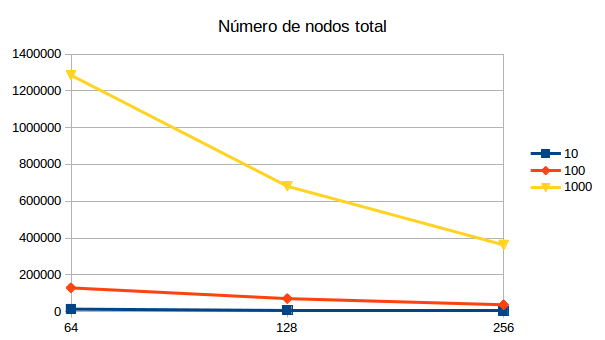
\includegraphics[width=12cm]{img/nodos-total}
	\caption{Número de nodos total para 64, 128 y 256 maps y 10, 100 y 1000 árboles}
	\label{fig:nodos-total}
\end{figure}

\subsubsection{Número de nodos promedio}

\begin{figure}[H]
	\centering
	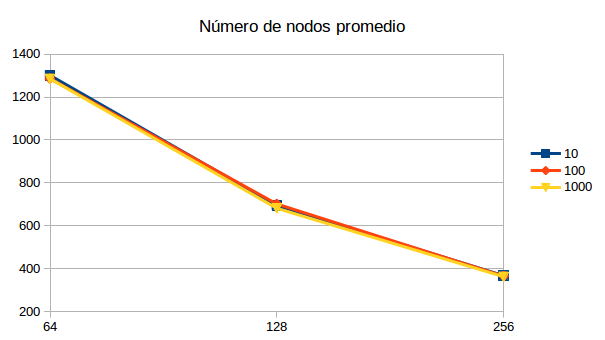
\includegraphics[width=12cm]{img/nodos-promedio}
	\caption{Número de nodos promedio para 64, 128 y 256 maps y 10, 100 y 1000 árboles}
	\label{fig:nodos-promedio}
\end{figure}

\subsubsection{Profundidad máxima del árbol}

\begin{figure}[H]
	\centering
	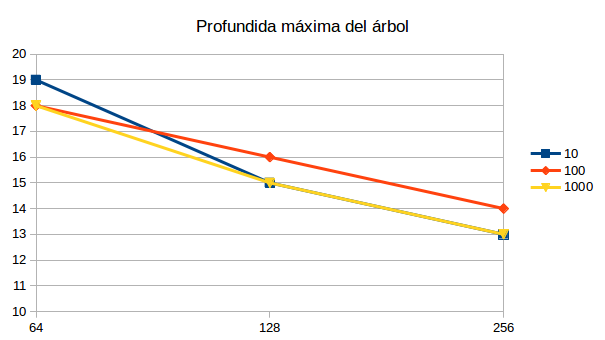
\includegraphics[width=12cm]{img/profundidad-maxima}
	\caption{Profundidad máxima para 64, 128 y 256 maps y 10, 100 y 1000 árboles}
	\label{fig:profundidad-maxima}
\end{figure}

\subsection{Tiempo de ejecución para entrenamiento}

\begin{figure}[H]
	\centering
	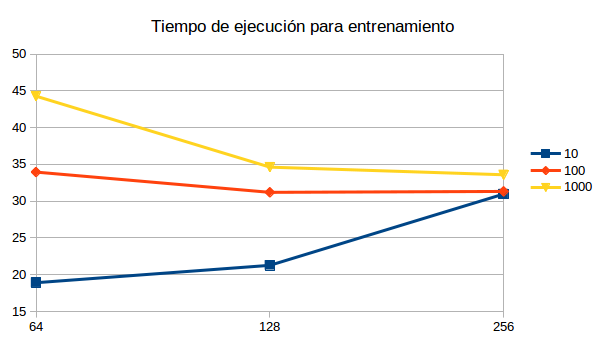
\includegraphics[width=12cm]{img/tiempo-entrenamiento}
	\caption{Tiempo de ejecución para entrenamiento para 64, 128 y 256 maps y 10, 100 y 1000 árboles}
	\label{fig:tiempo-entrenamiento}
\end{figure}

\subsection{Medidas de calidad}

\subsubsection{Accuracy estándar (test)}

\begin{figure}[H]
	\centering
	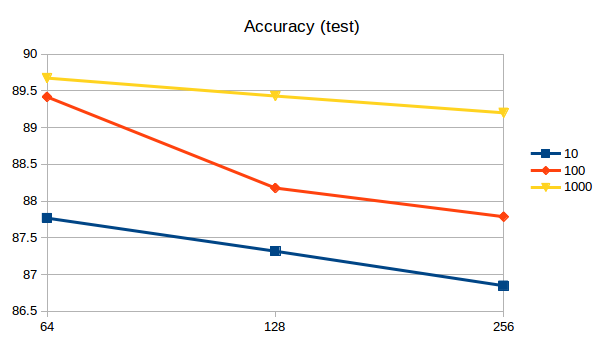
\includegraphics[width=12cm]{img/accuracy-test}
	\caption{Accuracy estándar sobre la partición de test para 64, 128 y 256 maps y 10, 100 y 1000 árboles}
	\label{fig:accuracy-test}
\end{figure}

\subsubsection{Accuracy estándar (training)}

\begin{figure}[H]
	\centering
	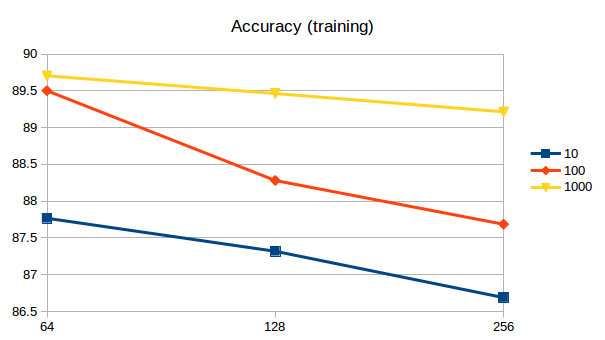
\includegraphics[width=12cm]{img/accuracy-training}
	\caption{Accuracy estándar sobre la partición de training para 64, 128 y 256 maps y 10, 100 y 1000 árboles}
	\label{fig:accuracy-training}
\end{figure}

\subsubsection{Media geométrica (test)}

\begin{figure}[H]
	\centering
	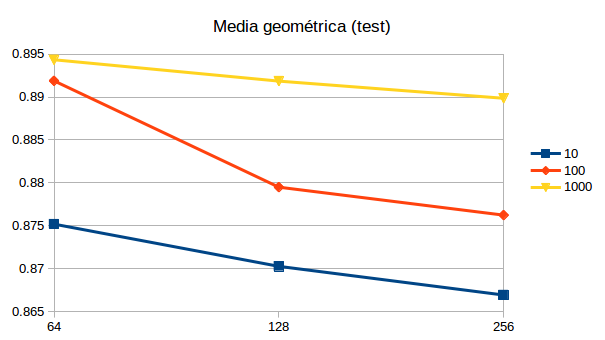
\includegraphics[width=12cm]{img/media-geometrica-test}
	\caption{Media geométrica sobre la partición de test para 64, 128 y 256 maps y 10, 100 y 1000 árboles}
	\label{fig:media-geometrica-test}
\end{figure}

\subsubsection{Media geométrica (training)}

\begin{figure}[H]
	\centering
	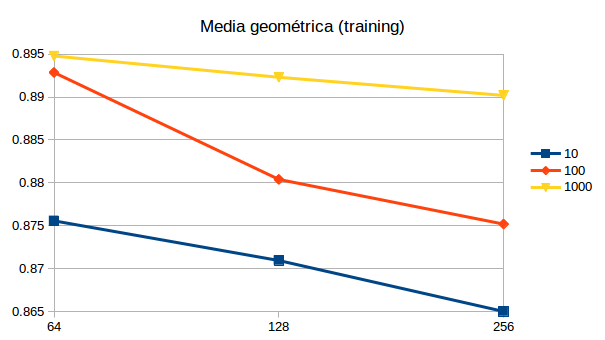
\includegraphics[width=12cm]{img/media-geometrica-training}
	\caption{Media geométrica sobre la partición de training para 64, 128 y 256 maps y 10, 100 y 1000 árboles}
	\label{fig:media-geometrica-training}
\end{figure}

%----------------------------------------------------------------------------------------
%	REFERENCIAS
%----------------------------------------------------------------------------------------

%\newpage

%\bibliography{referencias} %archivo referencias.bib que contiene las entradas 
%\bibliographystyle{plain} % hay varias formas de citar

\end{document}